\documentclass{article}
\usepackage{graphicx} % Required for inserting images
\usepackage[utf8]{inputenc}
\usepackage[backend=bibtex]{biblatex}
\addbibresource{references.bib}
\usepackage[T1]{fontenc}
\usepackage[polish]{babel}
\usepackage{amsmath,amssymb,amsthm}
\usepackage{float}
\usepackage{siunitx}
\usepackage{booktabs}
\usepackage{pgfplots}
\usepackage{geometry}
\usepackage{hyperref}
\usepackage{listings}
\usepackage{hyperref}
\lstset{ 
    language=Python, 
    basicstyle=\ttfamily\footnotesize, 
    keywordstyle=\color{blue}, 
    stringstyle=\color{black}, 
    commentstyle=\color{magenta}, 
    morecomment=[l][\color{black}]{\#}, 
    frame=single, 
    breaklines=true, 
    columns=fullflexible 
}
\usepackage{xcolor}
\geometry{a4paper, margin=1in}




\begin{document}
\begin{titlepage}
    \centering
    \vspace*{1cm}
    
    {\scshape\LARGE Uniwersytet w Białymstoku \par}
    \vspace{1.5cm}
    
    {\scshape\Large Wydział Fizyki \par}
    \vspace{1.5cm}
    
    {\huge\bfseries Sprawozdanie nr. 1 z ćwiczenia labolatoryjnego nr.24\\
    Temat: Badanie rozszerzalności cieplnej powietrza \\ \par}
    \vspace{2cm}
    
    {\Large\itshape Krzysztof Bezubik \par}
    \vspace{1cm}
    
    \begin{flushleft} 
    \large
    \textbf{Email:} kb89219@student.uwb.edu.pl \\
    \textbf{University:} Uniwersytet w Białymstoku \\
    \textbf{Department:} Wydział Fizyki \\
    \end{flushleft}
    
    \vfill
    
    {\large \today\par}
\end{titlepage}

\section{Cel ćwiczenia}
Celem ćwiczenia jest zbadanie jak zmienia się objętość powietrza pod wpływem zmian temperatury przy stałym ciśnieniu. 

\section{Wprowadzenie teoretyczne}

\textbf{Gaz doskonały} 

Gaz doskonały to model teoretyczny gazu, w którym zakłada się, że cząsteczki gazu nie oddziałują ze sobą i poruszają się zgodnie z prawami mechaniki klasycznej. W modelu tym pomija się objętość cząsteczek oraz siły międzycząsteczkowe.

\textbf{Równanie gazu doskonałego} 

Równanie stanu gazu doskonałego opisuje zależność między ciśnieniem ($P$), objętością ($V$) i temperaturą ($T$) gazu doskonałego:
\begin{equation}
    PV = nRT
\end{equation}
gdzie:
\begin{itemize}
    \item $P$ - ciśnienie [Pa]
    \item $V$ - objętość [m$^3$]
    \item $n$ - liczba moli [mol]
    \item $R$ - uniwersalna stała gazowa [$8.314 \frac{J}{mol \cdot K}$]
    \item $T$ - temperatura [K]
\end{itemize}

\textbf{Współczynnik rozszerzalności liniowej} 

Współczynnik rozszerzalności liniowej ($\alpha$) opisuje, jak zmienia się długość ciała stałego wraz ze zmianą temperatury:
\begin{equation}
    \alpha = \frac{1}{L} \frac{dL}{dT}
\end{equation}
gdzie:
\begin{itemize}
    \item $\alpha$ - współczynnik rozszerzalności liniowej [$\frac{1}{K}$]
    \item $L$ - długość początkowa [m]
    \item $dL$ - zmiana długości [m]
    \item $dT$ - zmiana temperatury [K]
\end{itemize}

\textbf{Współczynnik rozszerzalności objętościowej} 

Współczynnik rozszerzalności objętościowej ($\beta$) opisuje, jak zmienia się objętość ciała stałego lub cieczy wraz ze zmianą temperatury:
\begin{equation}
    \beta = \frac{1}{V} \frac{dV}{dT}
\end{equation}
gdzie:
\begin{itemize}
    \item $\beta$ - współczynnik rozszerzalności objętościowej [$\frac{1}{K}$]
    \item $V$ - objętość początkowa [m$^3$]
    \item $dV$ - zmiana objętości [m$^3$]
    \item $dT$ - zmiana temperatury [K]
\end{itemize}

\textbf{Współczynnik rozszerzalności objętościowej gazu doskonałego przy stałym ciśnieniu} 

Dla gazu doskonałego przy stałym ciśnieniu, współczynnik rozszerzalności objętościowej ($\beta$) jest odwrotnością temperatury:
\begin{equation}
    \beta = \frac{1}{T}
\end{equation}
gdzie:
\begin{itemize}
    \item $\beta$ - współczynnik rozszerzalności objętościowej [$\frac{1}{K}$]
    \item $T$ - temperatura [K]
\end{itemize}


\\
\hline
\\
\section{Omówienie pomiarów:}
Do realizacji ćwiczenia  potrzebowaliśmy by regularnie sprawdzać jak zmienia się poziom wody w odwróconej miarce (Rysunek.1 po lewej stronie oznaczone jako $V$) w skutek podgrzewania powietrza w zbiorniku $\textbf{V_{pwz}}$. Zanim rozpoczeliśmy zadanie zmierzyliśmy wartości początkowe:
\begin{itemize}
    \item $T_0$ = 22$^{\circ}$C
    \item $V_0$ = 154cm$^3$
    \item $\Delta T$ = 0,5$^{\circ}$C
    \item $\Delta V$ = 1cm$^3$
\end{itemize}

\begin{itemize}
    \item \textbf{Zmierzenie wartośći początkowych i niepewności urządzeń pomiarowych:} Do zmierzenia temperatury początkowej użyliśmy termometru rtęciowego o podziałce 0,1$^{\circ}$C. Do zmierzenia objętości początkowej użyliśmy odwróconej miarki o podziałce 2cm$^3$. Niepewność pomiaru temperatury wynosi 0,5$^{\circ}$C, a pomiaru objętości 1cm$^3$.
    \item \textbf{Podgrzewanie powietrza}: Powietrze w zbiorniku ($V_{pwz}$) podgrzewaliśmy za pomocą grzałki elektrycznej. W miarce odwróconej zanurzonej w wodzie obserwowaliśmy jak zmienia się poziom wody w miarce(w skutek wypychania jej w dół przez powietrze z góry) spisująć objętość z miarki co wzrost temperatury o 5 stopni Celsjusza.
    \item \textbf{Powtarzanie pomiarów:} Pomiary były wykonywane dla każdej objętości co zmiane temperatury $5^{\circ} C$. Po każdym pomiarze poprawialiśmy cylinder tak by poziom wody w środku cylindra był taki sam jak poziom wody w całym zbiorniku
\end{itemize}

\begin{figure}[H]
    \centering
    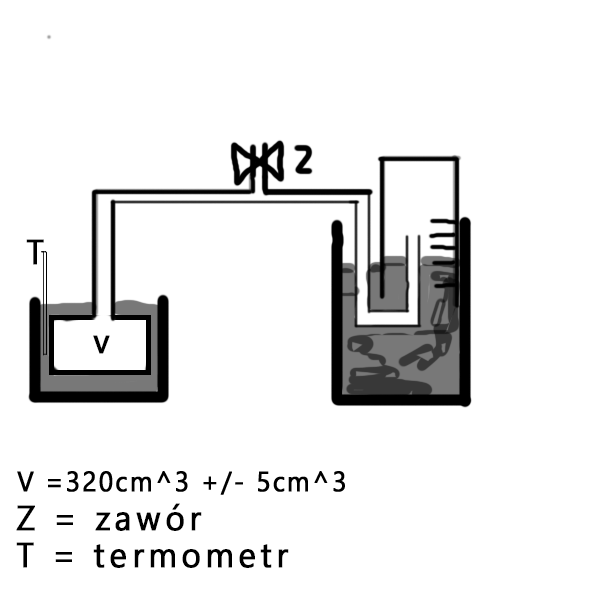
\includegraphics[width=0.75\linewidth]{zdjęcie1.png}
    \caption{Schemat układu pomiarowego}
    \label{fig:Rysunek_1}
\end{figure}

\section{Analiza pomiarów : }
Zebrane pomiary zapisałem w tabeli \ref{tab:pomiary}. Zakładamy że ciśnienie $[p = const]$ jest takie samo w całym zbiorniku, więc możemy zastosować równanie gazu doskonałego. W $V_pwz$ znajduje sie 
\
\begin{table}[h!]
    \centering
    \begin{tabular}{|c|c|c|c|c|}
    \hline
    \textbf{i} & \textbf{T\_i (*C)} & \textbf{T\_i (K)} & \textbf{V\_i (cm\textsuperscript{3})} & \textbf{V\_i (m\textsuperscript{3})} \\
    \hline
    1  & 28  & 301.15 & 160 & 0.00016 \\
    2  & 33  & 306.15 & 166 & 0.000166 \\
    3  & 38  & 311.15 & 170 & 0.00017 \\
    4  & 43  & 316.15 & 176 & 0.000176 \\
    5  & 48  & 321.15 & 180 & 0.00018 \\
    6  & 53  & 326.15 & 184 & 0.000184 \\
    7  & 58  & 331.15 & 188 & 0.000188 \\
    8  & 63  & 336.15 & 193 & 0.000193 \\
    9  & 68  & 341.15 & 197 & 0.000197 \\
    10 & 73  & 346.15 & 201 & 0.000201 \\
    11 & 78  & 351.15 & 205 & 0.000205 \\
    12 & 83  & 356.15 & 208 & 0.000208 \\
    13 & 88  & 361.15 & 212 & 0.000212 \\
    14 & 93  & 366.15 & 216 & 0.000216 \\
    15 & 98  & 371.15 & 220 & 0.00022 \\
    \hline
    \end{tabular}
    \caption{Tabela danych}
    \label{tab:tabela_danych}
    \end{table}




\subsection{Obliczanie niepewności}


Do obliczenia niepewnośći \ref{eq:l} $L_i$ również użyyjemy metody różniczki zupełnej której wzór wygląda następująco ($l_0$ ma stałą wartość wiec nie różniczkujemy po $l_0$) :
\begin{equation}
    \Delta L_i = |\frac{\partial L_i}{\partial l_i}| \cdot \Delta l_i
\end{equation}
\begin{equation}
    \Delta L_i = |-1|\cdot \Delta l_1
\end{equation}


\subsection{Obliczanie regresji liniowej}


\end{document}